\documentclass{ximera}
  \outcome{Interpret the accumulation function of speed as position}
  \outcome{Qualitatively evaluate net change from a graph}
  \outcome{Approximate displacement from velocity}
  \outcome{Track the changes in order to determine total change}
\begin{document}
\begin{problem}

  Car A and Car B are both going to drive from Columbus to
  Indianapolis, leaving Columbus at the same time.  The graph of the
  speed (in miles per hour) of the two cars is given below.  What is
  the relationship between the position of car $A$ and car $B$ after 2
  hours?

  \begin{image}
  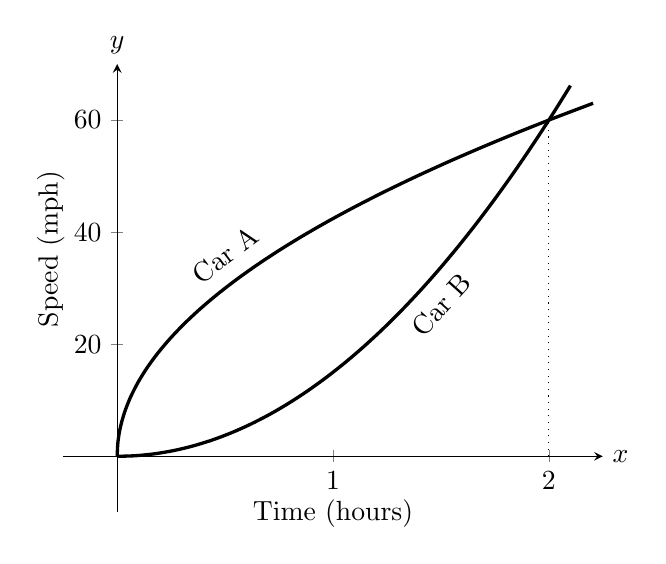
\begin{tikzpicture}
    \begin{axis}[
      clip=false,
      domain=-0:2.1, 
      ytick={20,40,60},
      xtick={1,2},
      ymin=-10, ymax=70,
      xmin=-0.25, xmax=2.25,
      xlabel=$x$, ylabel=$y$,
      axis lines=center,
      every axis y label/.style={at=(current axis.above origin),anchor=south},
      every axis x label/.style={at=(current axis.right of origin),anchor=west},
      axis on top,
      ]          
      \addplot [very thick,smooth] {30 * x^2/2};
      \addplot [very thick,smooth,domain=0:63] ({2*(x/60)^2},{x});
      \node at (axis cs:1,0) [anchor=north,yshift=-12pt] {Time (hours)};
      \node at (axis cs:0,37) [anchor=center,rotate=90,yshift=24pt] {Speed (mph)};
      
      \node at (axis cs:1.5,33) [anchor=center,yshift=-12pt,rotate=48] {Car B};
      \node at (axis cs:0.5,30) [anchor=center,yshift=12pt,rotate=37] {Car A};
      
      \draw [dotted] (axis cs:2,0) -- (axis cs:2,60);
    \end{axis}
  \end{tikzpicture}
  \end{image}

  \begin{multipleChoice}
    \choice[correct]{Car $A$ is ahead of car $B$.}
    \choice{Car $B$ is ahead of car $A$.}
    \choice{Car $B$ is passing car $A$.}
    \choice{Car $A$ and car $B$ are colliding.}
  \end{multipleChoice}
\end{problem}
\end{document}
